\documentclass[12pt,a4paper,usenames,dvipsnames]{article}
\usepackage[english]{babel}
\usepackage{aeguill}
\usepackage[T1]{fontenc}
\usepackage{txfonts}
\usepackage{graphicx}
\usepackage{latexsym}
\usepackage{url}
\usepackage{pdfpages}
\usepackage{color}
\usepackage{fancyhdr}
\usepackage[ocgcolorlinks,colorlinks=true,urlcolor=blue]{hyperref}
\usepackage[a4paper,margin=2cm]{geometry}
\usepackage{listings}
\usepackage{textcomp}

\renewcommand{\baselinestretch}{1.2}
\newcommand{\gratinversion}{0.3.1}
\newcommand{\gratintitle}{Gratin \gratinversion \  Documentation}
\newcommand{\addsection}[1]{{\color{Periwinkle}\section{#1}}}
\newcommand{\addsubsection}[1]{{\color{Periwinkle}\subsection{#1}}}
\newcommand{\addparagraph}[1]{{\vspace{0.3cm} \noindent \textbf{#1}}}

\newcommand{\addtitle}{
  \begin{center}
    \LARGE{\textbf{\expandafter\MakeUppercase\expandafter{\gratintitle}}}\\ \small{\today}
  \end{center}
}

\newcommand{\addauthors}{
  \begin{center}
    \begin{tabular}{cc}
      \large{Romain Vergne} & \large{Pascal Barla}
    \end{tabular}
  \end{center}
}

\newcommand{\remark}[1] {
  \begin{center}
    \fbox{  
      \begin{minipage}{0.9\textwidth}
         \color{orange}{#1}
      \end{minipage}
    }
  \end{center}
}
\newcommand{\todo}[1]{\textcolor{blue}{\emph{``#1''}}}

\pagestyle{fancy}
\fancyhead[L]{Gratin \gratinversion}
\fancyhead[C]{}
\fancyhead[R]{\today}

\lstdefinelanguage{GLSL}
{
sensitive=true,
morekeywords=[1]{
attribute, const, uniform, varying,
layout, centroid, flat, smooth,
noperspective, break, continue, do,
for, while, switch, case, default, if,
else, in, out, inout, float, int, void,
bool, true, false, invariant, discard,
return, mat2, mat3, mat4, mat2x2, mat2x3,
mat2x4, mat3x2, mat3x3, mat3x4, mat4x2,
mat4x3, mat4x4, vec2, vec3, vec4, ivec2,
ivec3, ivec4, bvec2, bvec3, bvec4, uint,
uvec2, uvec3, uvec4, lowp, mediump, highp,
precision, sampler1D, sampler2D, sampler3D,
samplerCube, sampler1DShadow,
sampler2DShadow, samplerCubeShadow,
sampler1DArray, sampler2DArray,
sampler1DArrayShadow, sampler2DArrayShadow,
isampler1D, isampler2D, isampler3D,
isamplerCube, isampler1DArray,
isampler2DArray, usampler1D, usampler2D,
usampler3D, usamplerCube, usampler1DArray,
usampler2DArray, sampler2DRect,
sampler2DRectShadow, isampler2DRect,
usampler2DRect, samplerBuffer,
isamplerBuffer, usamplerBuffer, sampler2DMS,
isampler2DMS, usampler2DMS,
sampler2DMSArray, isampler2DMSArray,
usampler2DMSArray, struct},
morekeywords=[2]{
radians,degrees,sin,cos,tan,asin,acos,atan,
atan,sinh,cosh,tanh,asinh,acosh,atanh,pow,
exp,log,exp2,log2,sqrt,inversesqrt,abs,sign,
floor,trunc,round,roundEven,ceil,fract,mod,modf,
min,max,clamp,mix,step,smoothstep,isnan,isinf,
floatBitsToInt,floatBitsToUint,intBitsToFloat,
uintBitsToFloat,length,distance,dot,cross,
normalize,faceforward,reflect,refract,
matrixCompMult,outerProduct,transpose,
determinant,inverse,lessThan,lessThanEqual,
greaterThan,greaterThanEqual,equal,notEqual,
any,all,not,textureSize,texture,textureProj,
textureLod,textureOffset,texelFetch,
texelFetchOffset,textureProjOffset,
textureLodOffset,textureProjLod,
textureProjLodOffset,textureGrad,
textureGradOffset,textureProjGrad,
textureProjGradOffset,texture1D,texture1DProj,
texture1DProjLod,texture2D,texture2DProj,
texture2DLod,texture2DProjLod,texture3D,
texture3DProj,texture3DLod,texture3DProjLod,
textureCube,textureCubeLod,shadow1D,shadow2D,
shadow1DProj,shadow2DProj,shadow1DLod,
shadow2DLod,shadow1DProjLod,shadow2DProjLod,
dFdx,dFdy,fwidth,noise1,noise2,noise3,noise4,
EmitVertex,EndPrimitive},
morekeywords=[3]{
gl_VertexID,gl_InstanceID,gl_Position,
gl_PointSize,gl_ClipDistance,gl_PerVertex,
gl_Layer,gl_ClipVertex,gl_FragCoord,
gl_FrontFacing,gl_ClipDistance,gl_FragColor,
gl_FragData,gl_MaxDrawBuffers,gl_FragDepth,
gl_PointCoord,gl_PrimitiveID,
gl_MaxVertexAttribs,gl_MaxVertexUniformComponents,
gl_MaxVaryingFloats,gl_MaxVaryingComponents,
gl_MaxVertexOutputComponents,
gl_MaxGeometryInputComponents,
gl_MaxGeometryOutputComponents,
gl_MaxFragmentInputComponents,
gl_MaxVertexTextureImageUnits,
gl_MaxCombinedTextureImageUnits,
gl_MaxTextureImageUnits,
gl_MaxFragmentUniformComponents,
gl_MaxDrawBuffers,gl_MaxClipDistances,
gl_MaxGeometryTextureImageUnits,
gl_MaxGeometryOutputVertices,
gl_MaxGeometryOutputVertices,
gl_MaxGeometryTotalOutputComponents,
gl_MaxGeometryUniformComponents,
gl_MaxGeometryVaryingComponents,gl_DepthRange},
morecomment=[l]{//},
morecomment=[s]{/*}{*/},
}

\lstset{
backgroundcolor=\color[rgb]{0.95, 0.95, 0.95},
tabsize=2,
rulecolor=,
basicstyle=\tiny,
upquote=true,
columns=fixed,
showstringspaces=false,
extendedchars=true,
breaklines=true,
prebreak = \raisebox{0ex}[0ex][0ex]{\ensuremath{\hookleftarrow}},
frame=single,
showtabs=false,
showspaces=false,
showstringspaces=false,
identifierstyle=\ttfamily,
keywordstyle=\color[rgb]{1.0,0,0},
keywordstyle=[1]\color[rgb]{0,0,0.75},
keywordstyle=[2]\color[rgb]{0.5,0.0,0.0},
keywordstyle=[3]\color[rgb]{0.127,0.427,0.514},
keywordstyle=[4]\color[rgb]{0.4,0.4,0.4},
commentstyle=\color[rgb]{0.133,0.545,0.133},
stringstyle=\color[rgb]{0.639,0.082,0.082},
}

\begin{document}
\begin{titlepage}
  \vspace*{\fill}
  \addtitle
  %
  \begin{figure}[h!]
    \centering
    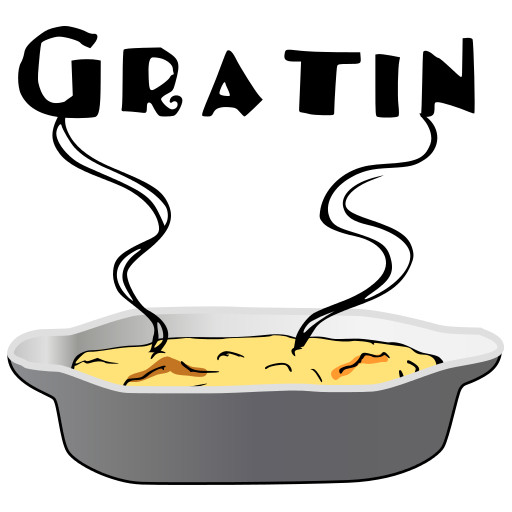
\includegraphics[width=0.5\linewidth]{imgs/gratin.jpg}
  \end{figure}
  %
  \addauthors
  \vspace*{\fill}
\end{titlepage}

\newpage
\tableofcontents
\newpage

\addsection{Gratin}
%
\addsubsection{Summary}
%
Gratin is a programmable node-based system tailored to the creation,
manipulation and animation of 2D/3D data in real-time on GPUs.
It is written in C++ and uses \href{http://www.qt.io/}{Qt}
for the interface, \href{http://eigen.tuxfamily.org/}{Eigen} for
linear algebra, \href{https://www.opengl.org/}{OpenGL} for renderings
and optionally \href{http://www.openexr.com/}{OpenExr} for loading and
saving high dynamic range images.  It is free and open source
(licensed under MPL v2.0) and relies on OpenGL and GLSL to ensure wide
OS and GPU compatibility.  Source code and installation packages are
available at \url{http://gratin.gforge.inria.fr/}.

\addsubsection{Contribute!}
You implemented a paper in Gratin, or you designed a useful node that
would benefit the graphics community? Please, send it to us, either as
a node (.grac file) or as a pipeline (.gra file). We will be pleased
to integrate it in the next release if possible. The nodes should come
with the author names, the citation of the paper (if there is a paper)
and a small description explaining how to use it.

\newpage
\addsection{Compilation}
Before all, make sure you have a GPU/graphics drivers capable to run (at least) OpenGL 4.1 applications. Otherwise, Gratin will not work. 

\addsubsection{Download sources}
Sources can be downloaded from the web site: \url{http://gratin.gforge.inria.fr/}, or via the svn repository:
\begin{lstlisting}[language=bash]{Name}
svn checkout https://scm.gforge.inria.fr/anonscm/svn/gratin/branches/gratin-v0.3.1 gratin
\end{lstlisting}

\addsubsection{Compiling on Debian, Ubuntu and Linux Mint}
\addparagraph{Install external packages}
\begin{lstlisting}[language=bash]{Name}
$ sudo apt-get install cmake qtbase5-dev libqt5svg5-dev libeigen3-dev libopenexr-dev
\end{lstlisting}

\addparagraph{Building Gratin}
\begin{lstlisting}[language=bash]{Name}
$ cd gratin
$ mkdir build
$ cd build
$ cmake ..
$ make -j4
\end{lstlisting}

\addparagraph{Launching Gratin}
\begin{lstlisting}[language=bash]{Name}
$ ./gratin [-in path/to/pipeline.gra]
\end{lstlisting}

\remark{Remark: Gratin will not compile if QT version is less than
  5.2. On old Linux distributions, QT5 might not be available
  natively. In that case, download and install from the web site:
  http://www.qt.io} 

\remark{Other Linux distributions: apart from the way
  external packages are installed, the installation should be
  equivalent.}

\addsubsection{Compiling on Mac OSX}

\noindent We provide an installation package for Mac OSX (Yosemite and later releases) on our Website: \\ \url{http://gratin.gforge.inria.fr/}.
Otherwise, Gratin may be compiled using the following steps.\\

\addparagraph{Install external packages}\\
Install required packages (Qt, OpenEXR, Eigen3) from the packaging system of Mac OS. 

\addparagraph{Building Gratin}
\begin{lstlisting}[language=bash,upquote=true]{Name}
$ cd gratin
$ mkdir build
$ cd build
$ cmake .. -DCMAKE_CXX_FLAGS='-DOPENGL_MAJOR_VERSION=4 -DOPENGL_MINOR_VERSION=1'
$ make -j4
\end{lstlisting}

\addparagraph{Launching Gratin}
\begin{lstlisting}[language=bash]{Name}
$ ./gratin [-in path/to/pipeline.gra]
\end{lstlisting}

\addsubsection{Compiling on Windows}
\noindent We provide a binary package for Windows 64 bits on our website:\\ \url{http://gratin.gforge.inria.fr/}.\\
\\ 
Otherwise, the simplest to compile Gratin is to use qtcreator: \url{http://www.qt.io/download/}. 
You should download and install all the required packages and open gratin/CMakeLists.txt via qtcreator. 
Once done, you should provide the paths to the libraries in the cmake options before building the solution. \\
\\
The main problem with the Windows compilation comes from the (optional) OpenEXR library that is quite difficult to obtain. It requires several weird steps that we do not describe here. 

\vspace{0.5cm}
\addsubsection{Cmake options}
\noindent A cmake error might be due to missing paths for the external
libraries. In that case, you must provide the good paths using
"-DLIBNAME\_\{INCLUDE/LIBRARY\}\_PATH", where LIBNAME is the name of the
missing library and INCLUDE or LIBRARY specifies if the target is a
source or a lib file. For instance, to specify the path to eigen, use:
\begin{lstlisting}[language=bash,upquote=true]{Name}
cmake -DEIGEN3_INCLUDE_DIR="path/to/eigen3" ..
\end{lstlisting}

\noindent If cmake does not find Qt, use the following option:
\begin{lstlisting}[language=bash,upquote=true]{Name}
cmake -DCMAKE_PREFIX_PATH="path/to/qt" ..
\end{lstlisting}

\noindent for changing the OpenGL version (default=4.2), use:
\begin{lstlisting}[language=bash,upquote=true]{Name}
cmake -DCMAKE_CXX_FLAGS='-DOPENGL_MAJOR_VERSION=4 -DOPENGL_MINOR_VERSION=1' ..
\end{lstlisting}
In that case, the version is set to OpenGL 4.1. 

\newpage
\addsection{Interface}
\begin{figure}[tbh]
  \centering
  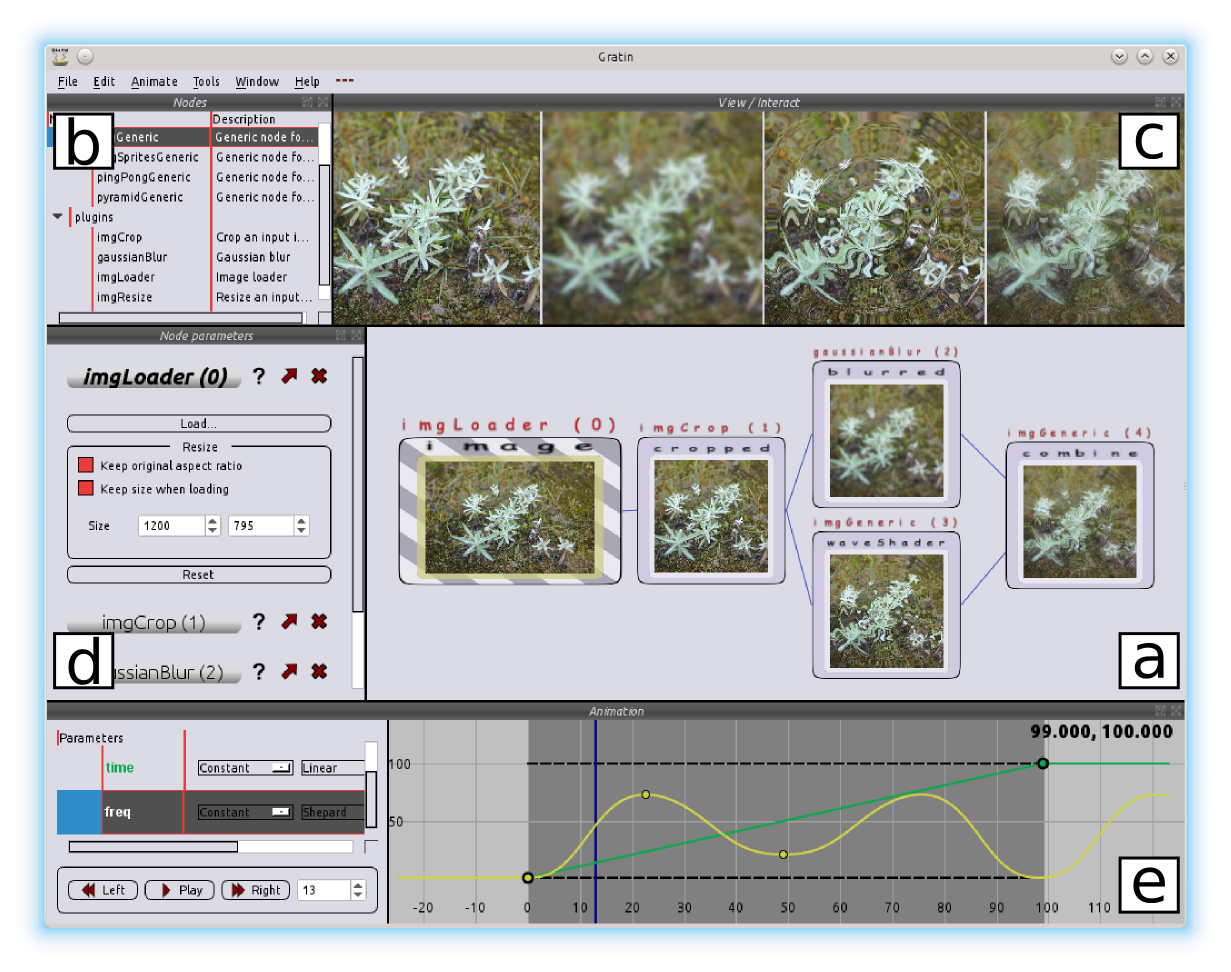
\includegraphics[width=\linewidth]{imgs/interface.png}
  \caption{\label{fig:interface}Interface of Gratin. (a) Graph
    visualization. (b) List of available nodes. (c) Node viewer. (d)
    Node interfaces. (e) Animation parameters and curves.}
\end{figure}

\noindent As shown in Figure~\ref{fig:interface}, the interface of our system
is composed of five main panels. The pipeline panel (a) where one can
interactively add, connect, disconnect, copy or paste nodes.  Node
outputs are visualized in real-time inside the interface.  All available nodes
are stored in user-defined directories and automatically loaded in the
node tree (b) at initialization.  The viewer (c) permits to display
particular node outputs and manipulate them via keyboard or mouse
events.  Each node has its own user-interface that can be displayed
and manipulated via a list of widgets (d).  Any node parameter may be
keyframed and interpolated via control curves in the animation panel
(e).

\newpage 

\addsubsection{Menu and global shortcuts}
\addparagraph{File menu}
\begin{itemize}
  \setlength\itemsep{0cm}
\item New (ctrl+n): clear everything. 
\item Open (ctrl+o): open an existing pipeline.
\item Save (ctrl+s): save/resave the current pipeline.
\item Save as: save the current pipeline in a new file.
\item Exit: quit the application. 
\end{itemize}

\addparagraph{Edit menu}
\begin{itemize}
 \setlength\itemsep{0cm}
\item Copy (ctrl+c): copy selected nodes inside the pipeline.
\item Paste (ctrl+v): paste selected nodes inside the pipeline.
\item Select all (ctrl+a): select/unselect all the nodes of the pipeline.
\item Reload: does nothing (only for debugging new implemented nodes).
\end{itemize}

\addparagraph{Animate menu}
\begin{itemize}
 \setlength\itemsep{0cm}
\item Play (p): start the animation. 
\item Stop (shift+p): stop the animation.
\item Next frame (shift+right): compute and show the next frame.
\item Previous frame (shift+left): compute and show the previous frame.
\item First frame (shift+up): compute and show the first frame.
\item Last frame (shift+down): compute and show the last frame.
\item Anim settings: choose the number of frames and the framerate. 
\end{itemize}

\addparagraph{Tools menu}
\begin{itemize}
 \setlength\itemsep{0cm}
\item Group (ctrl+g): group selected nodes (only if they form some directed acyclic graphs).
\item Ungroup (ctrl+shift+g): ungroup the selected node (only if the node is a group).
\item Export node output (ctrl+w): save a node output image (if an output is selected). 
\item Export node output animation (ctrl+shift+w): save all frames of a node output image (if an output is selected). 
\item Add node to list: if a node has been customized, this option allows the user to add the node inside the list of available nodes (panel b). The user has to choose a unique ID, a version, a name, a description and a help string that will be used for the new node. He also has to choose, in the list of available directories, the one in which the node will be saved. 
\item Manage node paths: allows the user to add or remove directories in which Gratin will look for new nodes when launched. This action needs a restart of Gratin. 
\end{itemize}

\addparagraph{Tools menu}
\begin{itemize}
 \setlength\itemsep{0cm}
\item Window/show-hide: show or hide panels (b), (c) and (d). 
\item Window/zoom: zoom/resize pipelines and images in panels (a) and (c).
\end{itemize}

\addparagraph{Help menu}
\begin{itemize}
 \setlength\itemsep{0cm}
\item Help: show the help widgets for all available nodes. 
\item About: display some information about Gratin. 
\end{itemize}

\addsubsection{Pipeline panel (a)}
\addparagraph{Summary of controls}
\begin{itemize}
 \setlength\itemsep{0cm}
\item Left click on a node: select it. If the click was done on an image, this action also selects the corresponding output inside the node. 
\item Double left click on a node: display its interface (panel d). 
\item Left click on the background : unselect all.
\item Left click, drag, drop on the background: select multiple nodes.
\item Right click, drag, drop on the background: move the scene.
\item Left click on an output, drag and drop on an input: create a connection. 
\item Wheel/middle click: zoom in/out.
\item Left click on a selected nodes, drag and drop: move selection.
\item Press space: add/remove a selected node output inside the viewer (panel c)
\item Press suppr: remove selection from the graph.
\end{itemize}

\addsubsection{Node panel (b)}
\noindent The node panel contains the tree of available nodes that can be added and combined inside the pipeline. A small description is also shown for each node. A double left click on a node will automatically insert it inside the graph. 

\vspace{0.5cm}
\addsubsection{Viewer panel (c)}
\addparagraph{Summary of controls}
\begin{itemize}
 \setlength\itemsep{0cm}
\item Left click on an image: select the corresponding node. 
\item mouse/keyboard on top of a selected node: interact with the node (depends on the node).
\item Left click on the background / press esc: unselect everything.
\item Right click, drag, drop on the background: move the scene.
\item Wheel/middle click: zoom in/out. 
\item Press suppr: remove selected node from the viewer. 
\item Press ctrl+right: move selected node to the right.
\item Press ctrl+left: move selected node to the left.
\end{itemize}

\addsubsection{Node interface (d)}
\begin{figure}[tbh]
  \centering 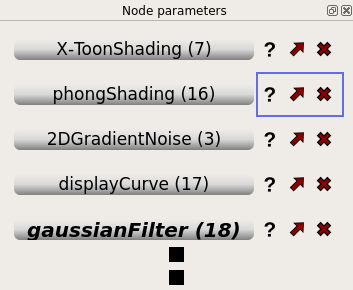
\includegraphics[width=0.4\linewidth]{imgs/node-param.png} 
  \caption{\label{fig:node-param}Each
  node interface is displayed as a list of widgets in the panel d. }
\end{figure}
\noindent The panel d contains a list of node interfaces opened by the user (via a double click on a node), as shown in Figure~\ref{fig:node-param}. Each widget thus contains parameters specific to each node as well as 3 buttons (as shown in the blue square):
\begin{itemize}
 \setlength\itemsep{0cm}
\item a help button (showing a small widget containing the documentation of this particular node),
\item a detach button (detach the window - useful when programming inside the interface),
\item a close button that removes this interface from the list (simply double-click again on the node to show it again). 
\end{itemize}
%
\begin{figure}[tbh]
  \centering 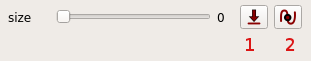
\includegraphics[width=0.4\linewidth]{imgs/one-param.png} 
  \caption{\label{fig:one-param}A keyframable parameter.}
\end{figure}
Each parameter contained in the node interface might be animated using keyframed curves. A keyframed parameter can be easily recognized by its associated 2 buttons, as shown in Figure~\ref{fig:one-param}:
 \begin{enumerate}
 \setlength\itemsep{0cm}
\item create a keyframe at the current frame with the chosen value inside the interface. 
\item Add the parameter inside the animation panel (d) in order to control its curve(s). 
\end{enumerate}


\addsubsection{Animation panel (e)}
\begin{figure}[tbh]
  \centering 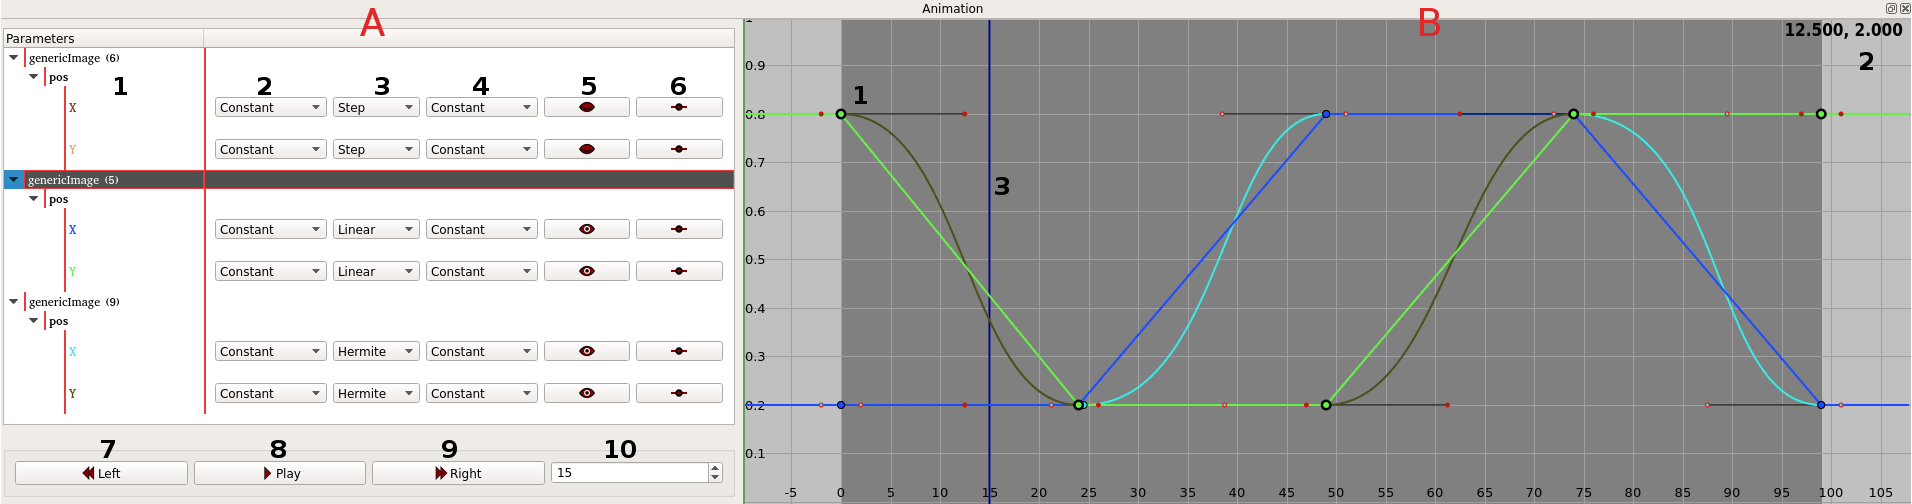
\includegraphics[width=1\linewidth]{imgs/anim-widget.png} 
  \caption{\label{fig:anim-widget}The animation panel}
\end{figure}
\noindent The animation panel is composed of 2 main widgets, as shown in Fig.~\ref{fig:anim-widget}. The first one (A) contains the list of parameters currently edited by the user, their options and the player. The second one (B) shows the corresponding keyframed curves that can be edited directly. 

\addparagraph{A: list of parameters}
\begin{enumerate}
 \setlength\itemsep{0cm}
\item parameters are displayed in a tree widget, containing the node name (root), the parameter name and each of its components. 
\item control the behavior of the curve before the first control point (see Fig.~\ref{fig:curves}). 
\item control the type of interpolation used in-between control points (see Fig.~\ref{fig:curves}). 
\item control the behavior of the curve after the last control point (see Fig.~\ref{fig:curves}). 
\item show/hide the curve in widget B.
\item clear all control points for this curve.
\item (shift+up) place the current frame at the beginning of the animation.
\item (p and shift+p) play/stop the animation 
\item (shift+down) place the current frame at the end of the animation.
\item show and select the current frame.
\end{enumerate}
Available curve behaviors and types are summarized in Fig.~\ref{fig:curves}. 

\begin{figure}[htb]
 \centering
\begin{tabular}{@{} c @{\hspace{4pt}} c @{\hspace{4pt}} c @{\hspace{4pt}} c @{\hspace{4pt}} c @{\hspace{4pt}} c @{}}
 & \tiny{Constant} & \tiny{Linear} & \tiny{Repeat} & \tiny{Offsetted} & \tiny{Mirrored}\\
 \rotatebox[origin=c]{90}{\rlap{\tiny{Linear}}}&
 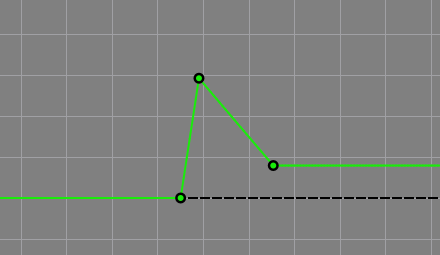
\includegraphics[width=0.19\linewidth]{imgs/kf01.png}&
 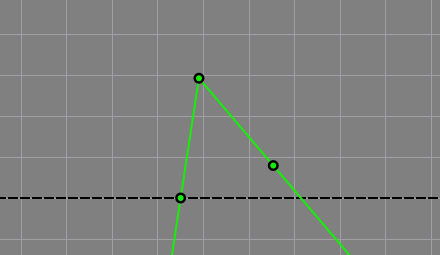
\includegraphics[width=0.19\linewidth]{imgs/kf06.png}&
 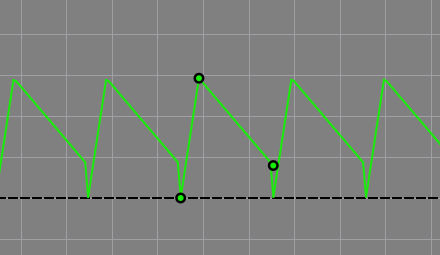
\includegraphics[width=0.19\linewidth]{imgs/kf11.png}&
 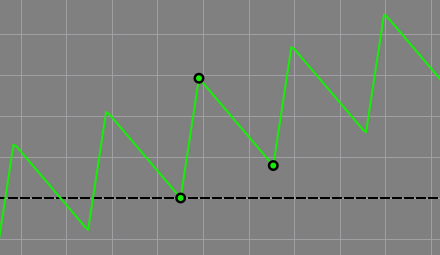
\includegraphics[width=0.19\linewidth]{imgs/kf16.png}&
 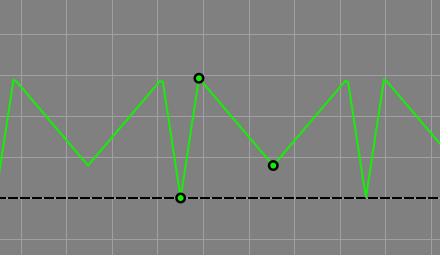
\includegraphics[width=0.19\linewidth]{imgs/kf21.png}\\
 \rotatebox[origin=c]{90}{\rlap{\tiny{Step}}}&
 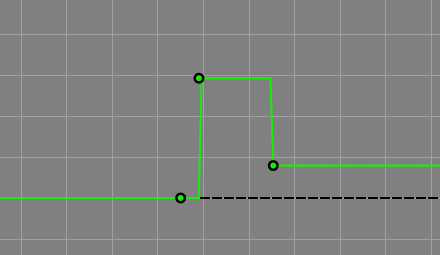
\includegraphics[width=0.19\linewidth]{imgs/kf02.png}&
 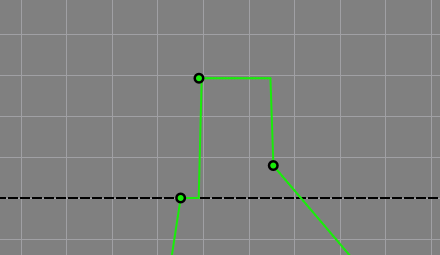
\includegraphics[width=0.19\linewidth]{imgs/kf07.png}&
 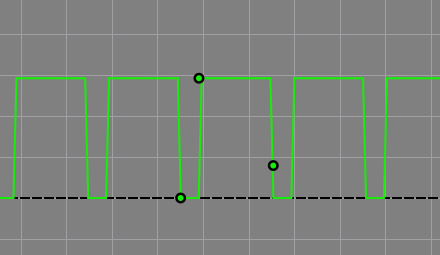
\includegraphics[width=0.19\linewidth]{imgs/kf12.png}&
 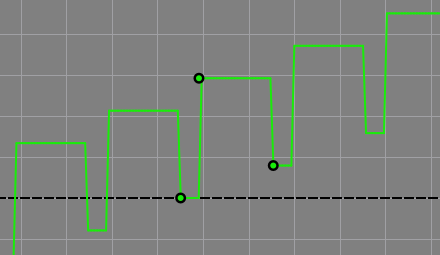
\includegraphics[width=0.19\linewidth]{imgs/kf17.png}&
 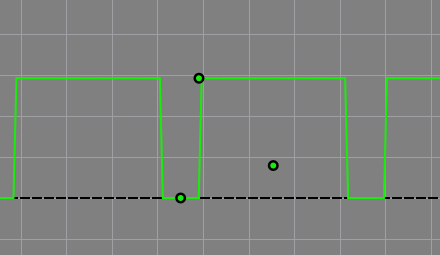
\includegraphics[width=0.19\linewidth]{imgs/kf22.png}\\
 \rotatebox[origin=c]{90}{\rlap{\tiny{Shepard}}}&
 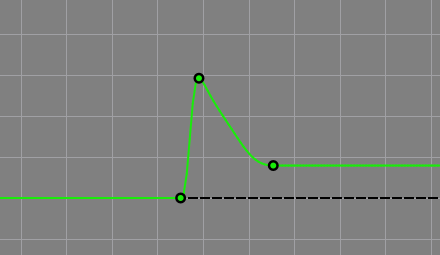
\includegraphics[width=0.19\linewidth]{imgs/kf03.png}&
 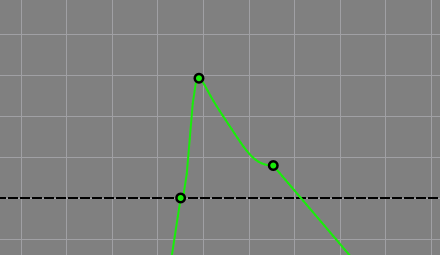
\includegraphics[width=0.19\linewidth]{imgs/kf08.png}&
 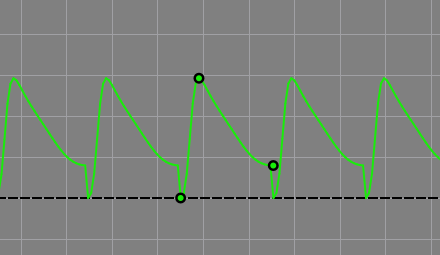
\includegraphics[width=0.19\linewidth]{imgs/kf13.png}&
 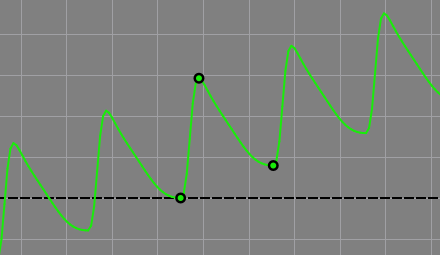
\includegraphics[width=0.19\linewidth]{imgs/kf18.png}&
 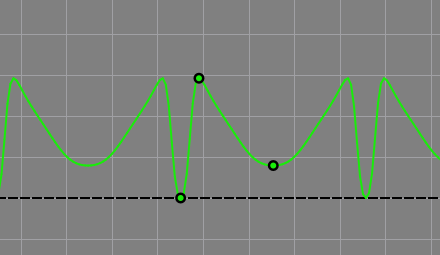
\includegraphics[width=0.19\linewidth]{imgs/kf23.png}\\
 \rotatebox[origin=c]{90}{\rlap{\tiny{Spline}}}&
 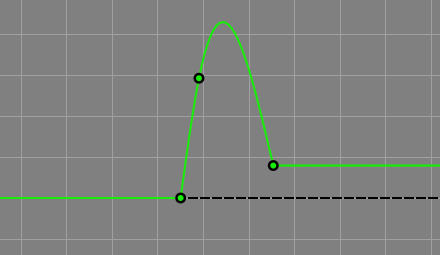
\includegraphics[width=0.19\linewidth]{imgs/kf04.png}&
 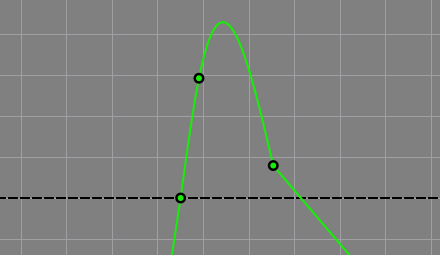
\includegraphics[width=0.19\linewidth]{imgs/kf09.png}&
 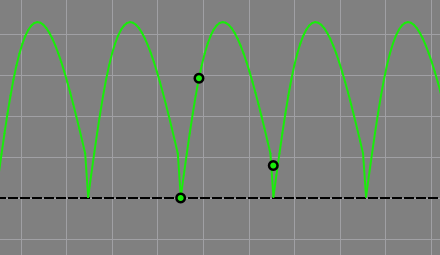
\includegraphics[width=0.19\linewidth]{imgs/kf14.png}&
 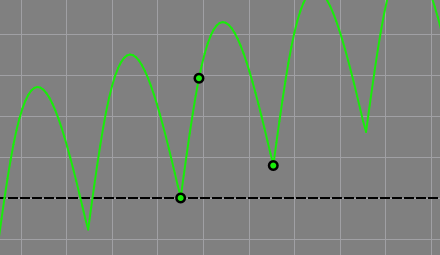
\includegraphics[width=0.19\linewidth]{imgs/kf19.png}&
 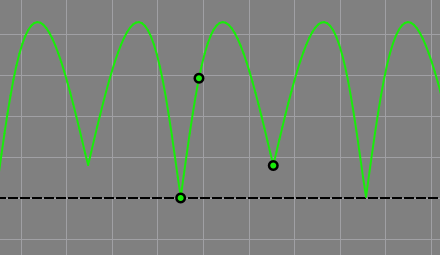
\includegraphics[width=0.19\linewidth]{imgs/kf24.png}\\
 \rotatebox[origin=c]{90}{\rlap{\tiny{Hermite}}}&
 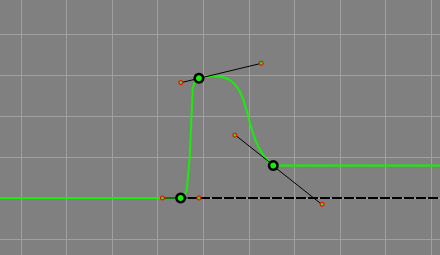
\includegraphics[width=0.19\linewidth]{imgs/kf05.png}&
 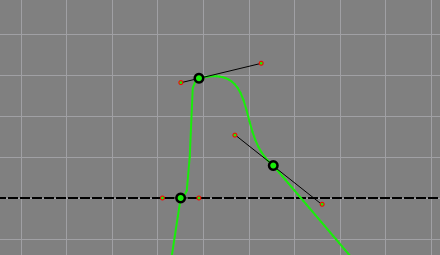
\includegraphics[width=0.19\linewidth]{imgs/kf10.png}&
 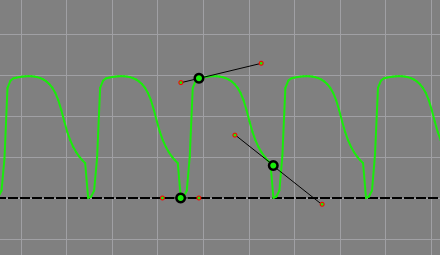
\includegraphics[width=0.19\linewidth]{imgs/kf15.png}&
 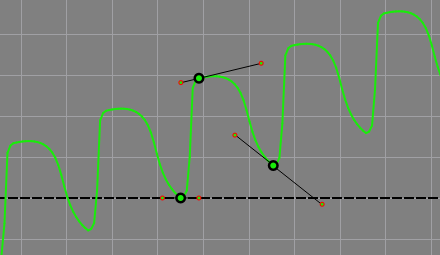
\includegraphics[width=0.19\linewidth]{imgs/kf20.png}&
 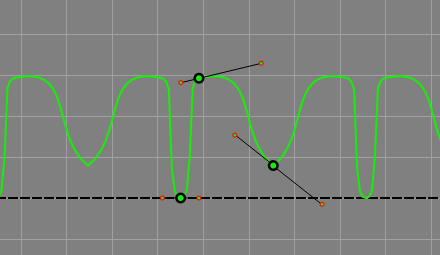
\includegraphics[width=0.19\linewidth]{imgs/kf25.png}
 \end{tabular}
\caption{\label{fig:curves}
Curve types and behaviors obtained with three control points. 
The y-axis shows the types of interpolation implemented in our system. 
The x-axis shows the modes controlling the behavior of the curves before and after the first and last control points. }
\end{figure}

\addparagraph{B: curve edition}

\noindent All selected curves can be visualized and edited in widget B. Control points are displayed with small dots (1). Their positions are displayed on the top right corner (2). The current frame is also displayed with a blue line (3). Here is a summary of the controls in this widget:
\begin{itemize}
 \setlength\itemsep{0cm}
\item Left click on the frame bar and drag: modify the current frame. 
\item Left click on a control point: select the corresponding curve. 
\item Left click on a control point and drag: modify the position of the control point. 
\begin{itemize}
 \setlength\itemsep{0cm} 
 \item +ctrl: use big steps to control the position. 
 \item +shift: use small steps to control the position. 
\end{itemize}
\item Ctrl+right click on the background: add a control point to the selected curve.
\item Ctrl+middle click on a control point: remove the control point from the selected curve.
\item Right click on the background: move the scene.
\item Wheel: zoom in/out.
\item Ctrl+wheel/middle click and drag horizontally: horizontal scaling.
\item Shift+wheel/middle click and drag vertically: vertical scaling.
\end{itemize}

\newpage
\addsection{Programming generic nodes}

\begin{figure}[htb]
  \centering 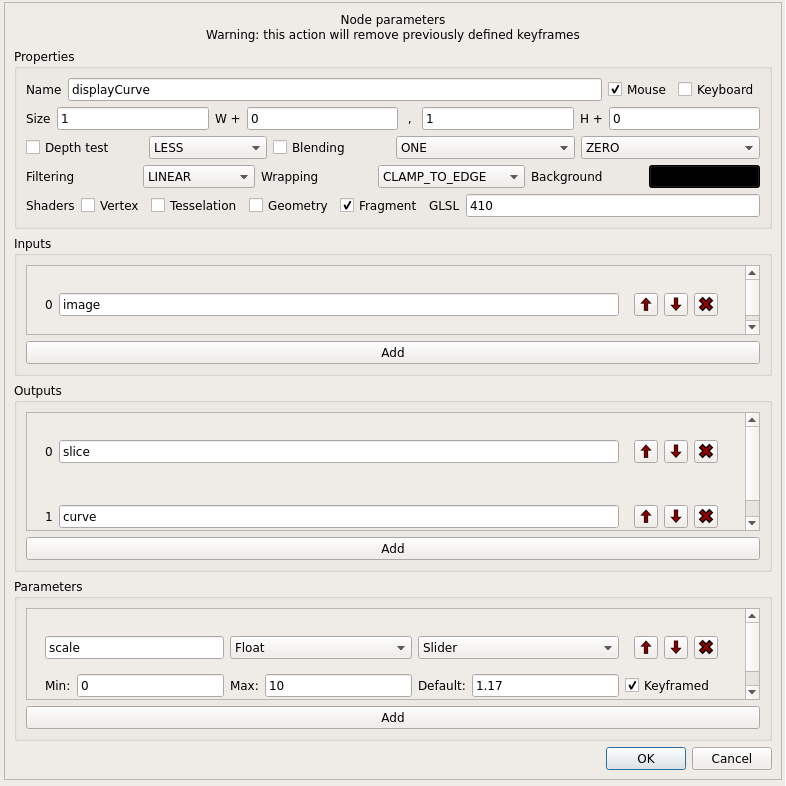
\includegraphics[width=\linewidth]{imgs/generic-settings.png} 
  \caption{\label{fig:generic-settings}Settings of a generic node.}
\end{figure}

\noindent Generic nodes provide users with the ability to precisely customize
processes to their needs by writing GLSL shaders directly from inside
the user interface. Most of the nodes available in Gratin are in fact
designed with generic nodes and their code might be directly modified
by users.  The creation of a generic node begins with the filling of a
dialog box where users specify important parameters of a GLSL shader
(Fig.~\ref{fig:generic-settings}):
\begin{itemize}
 \setlength\itemsep{0cm}
\item Properties: contains the name and other general parameters for
  the node. Check mouse and/or keyboard will grant access to mouse
  positions and keyboard keys in the shaders. The size of the output
  images are chosen via a function of the input texture sizes W and H
  (0 if no input). The user may also enable the depth test (with
  commonly used OpenGL functions), the blending, the filtering and the
  wrapping used for the output textures (see the OpenGL documentation
  - \url{https://www.opengl.org/} - for more information on how these
  options will affect the resulting images). Finally, the user can
  decide which shaders to activate
  (vertex/tesselation/geometry/fragment), choose the GLSL version and
  a default background color.
\item Inputs/outputs: choose the number of input
  (resp. output) images and modify their names. Chosen names will be
  directly used inside the shaders.
\item Parameters: add/remove necessary parameters. For each
  parameter, one may choose a name, a type (int/float/vec2/etc) and
  how it should appear in the node interface (slider/spin/etc). Min,
  max and default values should also be provided. Finally, checking
  the keyframed checkbox will allow the parameter to be controlled by
  keyframe curves.
\end{itemize}
%
Once the settings have been chosen, users may customize the node behavior
by writing GLSL code and observing results in real-time. Input and
output names are used to automatically generate the head of the
shaders. All the parameters are also available via generated uniform
variables. In the following, we present the different types of generic
nodes currently available in Gratin. For more information about how to
program using GLSL, visit:
\url{https://www.opengl.org/documentation/glsl/}. The provided
pipeline samples also illustrate how each of these generic node has
been used to produce different effects.

\remark{Remark: modifying the settings of a node will remove all previously defined keyframes for this node} 
% Romain: Je me rappelle plus pourquoi on avait mis ca et je comprend pas: and make also make shaders incorrect.}

\addsubsection{Generic image node} 
%
This node permits to analyze, manipulate and visualize input textures
(e.g., colored images, g-buffers).  As commonly done for image
processing in OpenGL, a simple quad is drawn in the viewport so that
input textures can be easily accessed and mapped to create outputs
containing specific effects.  This node may be used to create one-pass
custom complex shaders (as in
\href{https://www.shadertoy.com/}{Shadertoy} for instance), to mix
input images, to create various patterns and so on.
Implementation-wise, user-specified GLSL version, input and output
texture names are automatically used to generate the header of the
shader.  By default, the fragment shader simply makes a copy of the
first input texture.

\vspace{0.5cm}
\addsubsection{Generic buffers and grid nodes}
They let users apply
any effect to 3D meshes by customizing vertex, tessellation, geometry
and fragment shaders.  The main difference between object and grid
node types is that the former loads a mesh in OBJ format, while the
latter creates a planar grid.  In the case of the grid node,
tessellation is chosen by the user in the dedicated interface;
vertices are then typically displaced according to input GLSL code.
As with other generic nodes, any number of textures might be provided
as input (such as color or normal maps for instance).  Outputs are
typically in the form of g-buffers or renderings for further 3D or 2D
processing respectively.  A trackball camera is associated to this
node so that users may manipulate their object in the viewer panel.
In both cases, mesh positions, normals, tangents and texture
coordinates are directly sent as vertex attributes.  Consequently, the
header of the vertex shader is adapted to grant access to these
attributes.

\vspace{0.5cm}
\addsubsection{Generic splat node} 
This node permits to manipulate point
sprites and is useful to control particles, visualizations or even
image warpings.  The particularity here is to be able to modify splat
sizes and locations (possibly using overlapping and blending) to
obtain specific effects.  The interface permits to control the number
of rendered sprites, and their behavior is controlled through GLSL
code.  In practice, it works by sending a set of point sprites to the
GPU, with one splat per pixel by default.  Shader headers for the
generic splat node contain the position of the splat (as an attribute
in the vertex shader), as well as uniform variables.  The remainder of
the shader can be freely modified.

\vspace{0.5cm}
\addsubsection{Generic pyramid node} 
%
This node creates one or more mipmaped textures where one can control
how each level is computed.  It might be used for the creation of
usual mipmaps, but also for multiscale analysis (Gaussian or Laplacian
pyramids) or to compute global information such as the mean and
variance of an input image.  The shader header is automatically
generated and contains variables such as the number of levels and
flags to know whether the top or bottom of the pyramid have been
reached.  In addition, the previously computed level of each input
texture is automatically added to the GPU program as a uniform
sampler.  Users thus only have to describe per-level operations in a
specific order (top-down or bottom-up) in the GLSL code.  The
resulting pyramids are stored as mipmaps.  Further connected nodes may
thus easily access any texture level via GLSL built-in functions such
as \textit{textureLod()}.

\vspace{0.5cm}
\addsubsection{Generic ping-pong node} 
%
This node provides another useful feature commonly used in GPU
programming to implement iterative processes.  The same process is
applied at each internal pass, and repeated a number of times
specified by the user.  Such a type of node may be used to iteratively
accumulate or propagate some information in the output textures.  In
practice, it uses a pair of textures for internal multiple passes,
with one texture being read and the other written on even passes, and
the opposite on odd passes.  However, this is not apparent to the
user: we automatically generate a header that gives access to the
resulting texture of the previous internal pass, as well as the
current pass number.  Note that such a ping-pong architecture could
not be created manually by connecting simpler nodes, since our graph
is acyclic.

\remark{Remark: when opening a pipeline containing a ping-pong node, it will by default be initialized and run for the default number of passes. 
This might lead to important lags when each pass is a time-consuming process.} 


\newpage
\addsection{Pipeline samples} 
%
\noindent A good start for designing new pipelines
is to have a look at and take inspiration from the provided samples
available in ``data/pipes''. They describe how to use generic nodes
and show how to easily and quickly obtain multiple effects. This
section presents the samples.

\addsubsection{image-operators.gra}
%
\begin{figure}[htb]
  \centering 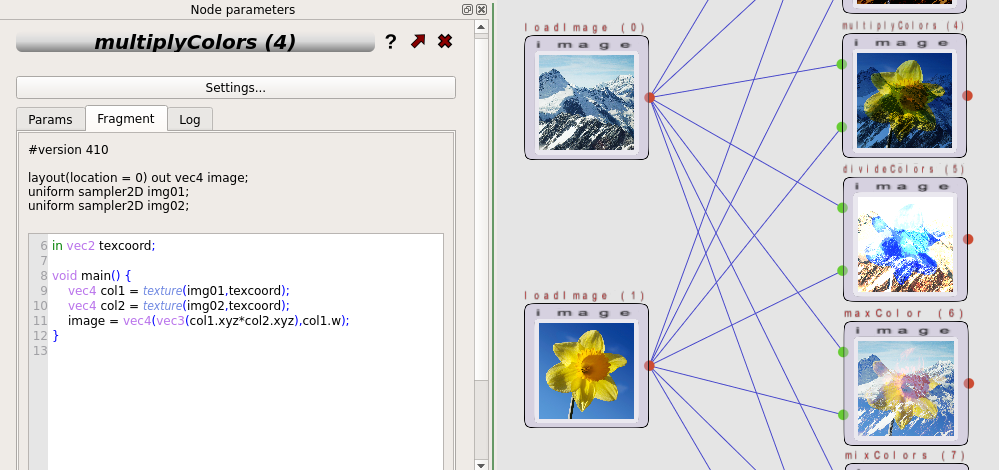
\includegraphics[width=\linewidth]{imgs/pipe-img-operators.png} 
  \caption{\label{fig:pipe-opp}The image operator pipeline example.}
\end{figure}
%
\noindent image-operators is the simplest pipeline and shows how to
combine two input images using simple image operators ($+,-,*,/,etc$).
Images are loaded with a ``loadImage'' node. All the combining
operations are done with some ``genericImage'' nodes
(Fig.~\ref{fig:pipe-opp}). In these nodes, the fragment shader is
executed independently on each image pixel. One can visualize the code
by double-clicking on a node and choosing the ``fragment'' tab in the
node interface. Of course, you can modify the settings and the code to
obtain your own desired effect. The only node containing a parameter
in these examples is the ``mixColors'' node that linearly interpolates
between 2 images based on a user-chosen value (in the ``Params'' tab
of the node interface).

\addsubsection{color-conversion.gra}
%
\begin{figure}[htb]
  \centering 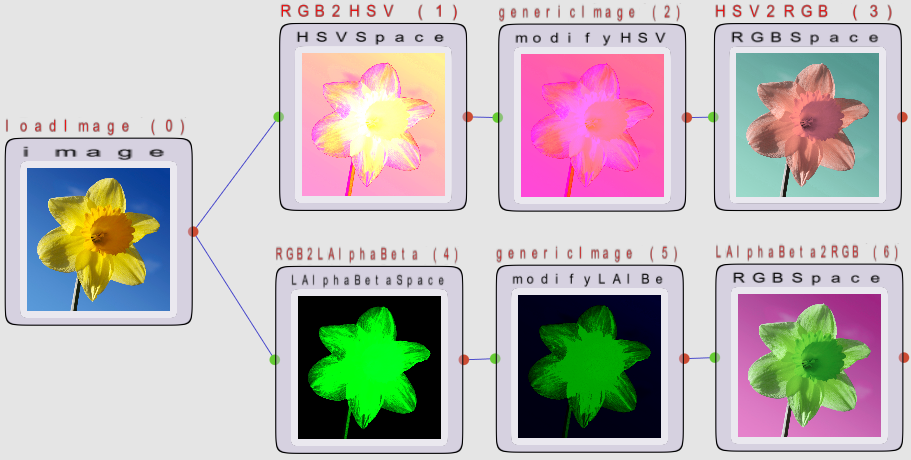
\includegraphics[width=\linewidth]{imgs/pipe-color-conv.png} 
  \caption{\label{fig:pipe-col-conv}The color conversion pipeline example.}
\end{figure}
%
\noindent This pipeline illustrates the use of color conversion nodes
to manipulate image colors (Fig.~\ref{fig:pipe-col-conv}). Except for the
loader, all nodes were created from the genericImage node. The top
row first convert an input RGB image into the HSV color space. A node
is then provided to control and manipulate HSV parameters (double
click on the ``modifyHSV'' node to try it via the interface). The last
node convert the HSV color back to the RGB color space, so that the
image can be displayed properly. The bottom row is similar, except
that colors are converted into the $L\alpha\beta$ color space.

\newpage
\addsubsection{image-filtering.gra}
%
\begin{figure}[b!]
  \centering 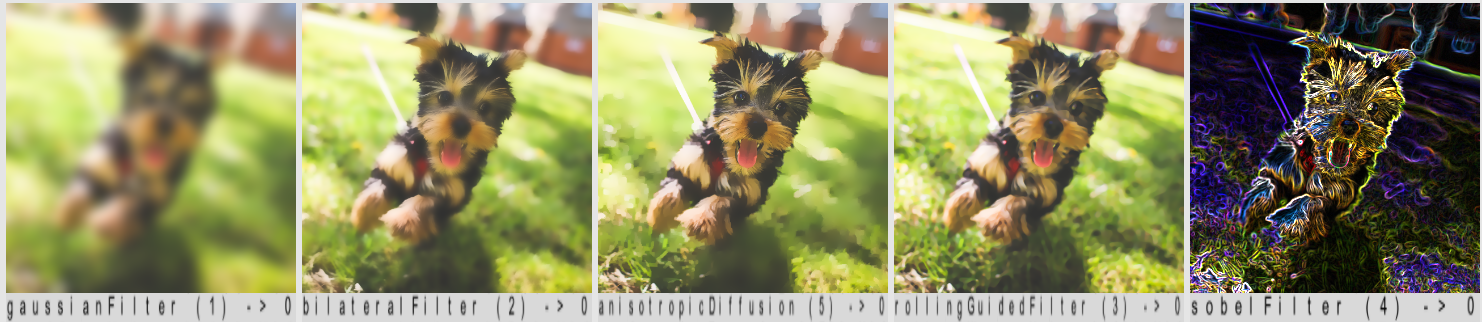
\includegraphics[width=\linewidth]{imgs/pipe-filter.png} 
  \caption{\label{fig:pipe-filter}Image filtering pipeline example.}
\end{figure}
%
\noindent This pipeline (Fig.~\ref{fig:pipe-filter}) illustrates the use of currently available
filtering nodes. The gaussian filter (left) was not implemented in a
generic node because it was optimized with a two-pass convolution kernel. The
bilateral filter (second) is based on a genericImage node. The
intensity and spatial sigma parameters can be controlled in the node
interface. The third example shows how a genericPingPong node was used
to obtain an anisotropic diffusion that iteratively diffuse colors
everywhere except on edges. The fourth example uses the same process
to obtain the rolling guided filter. The fifth example is based on a
genericImage node and detects edges using a Sobel filter.
\remark{Remark: citations for implemented papers are provided inside the node
  descriptions/helps.}

\addsubsection{curves-surfaces.gra}
\begin{figure}[htb]
  \centering 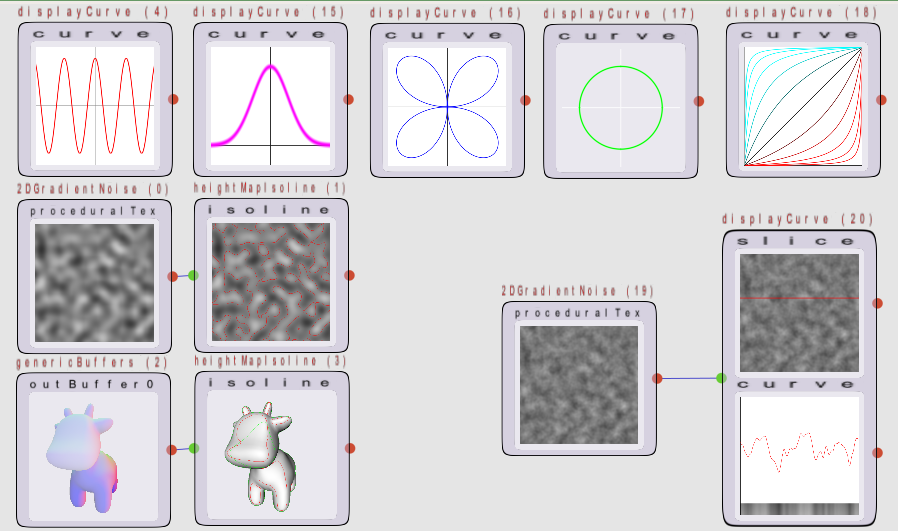
\includegraphics[width=\linewidth]{imgs/pipe-curves01.png} 
  \caption{\label{fig:pipe-curves}The curves examples.}
\end{figure}
%
\noindent This pipeline shows how to use nodes to visualize isolines,
curves and surfaces. The node ``displayCurve'' is based on a
genericImage node. It allows the user to easily modify a function
inside the GLSL code and visualize the resulting curve. The top row of
Fig.~\ref{fig:pipe-curves} shows some variations of this node, with
different functions, thicknesses and colors. To set your own curve,
open the ``fragment'' tab inside the node interface and modify the
equation inside the ``evalFunc'' function. Any parameter may be added
to the interface to control the curves in real-time, as shown in the
sine function node. \\ \\
%
In the bottom left of the figure, 2 examples of isoline visualization
are given. Again, this node is based on a genericImage node and might
be modified depending on user expectations. The first example shows
the isoline on a 2D noise texture. The isovalue can be controlled
inside the node interface. In the second example, the GLSL code was
slightly modified to simultaneously show 2 isoline curves, based on
2.5D information as input (surface slant in red and depth in Green).\\
\\
%
Finally, the bottom right example is a variation of the
``displayCurve'' node that was modified to display a slice of an input
image. This slice can be interactively changed in the viewer panel:
click on the slice and associated curve image and press ``space'' on
both of them. The two node outputs should thus appear in the viewer
panel. In this viewer, click on the slice image to select it and click
and drag vertically to control which slice to display in the curve
image.
%
\begin{figure}[htb]
  \centering 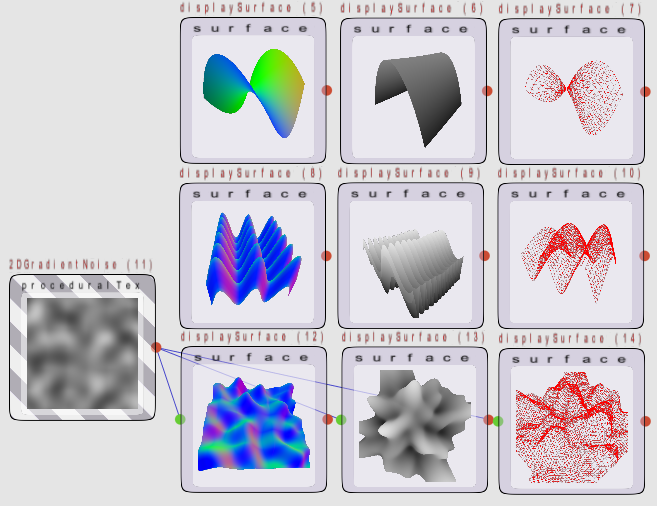
\includegraphics[width=\linewidth]{imgs/pipe-curves02.png} 
  \caption{\label{fig:pipe-surf}The surfaces examples.}
\end{figure}
% 
This pipeline also contain a set of nodes for visualizing surfaces, as
shown in Fig.~\ref{fig:pipe-surf}.  All these nodes are actually based
on variations of the ``displaySurface'' node, itself based on a
``genericGrid'' node. The user may modify the surface function by
editing the ``evalFunc'' function inside the vertex tab of the node
interface. From left to right, surfaces are visualized with their
normals (surface orientation), height and in wireframes. The top row
shows a quadratic function that can be manipulated with 2
parameters. The second row is a sinewave surface. The third one used a
heightfield as input to generate the 3D surface. The scale parameter
of the interface allows the height to be scaled manually. The camera
can be controlled in the viewer for each of this node.

\newpage
\addsubsection{flow-visualization.gra}
%
\begin{figure}[htb]
  \centering 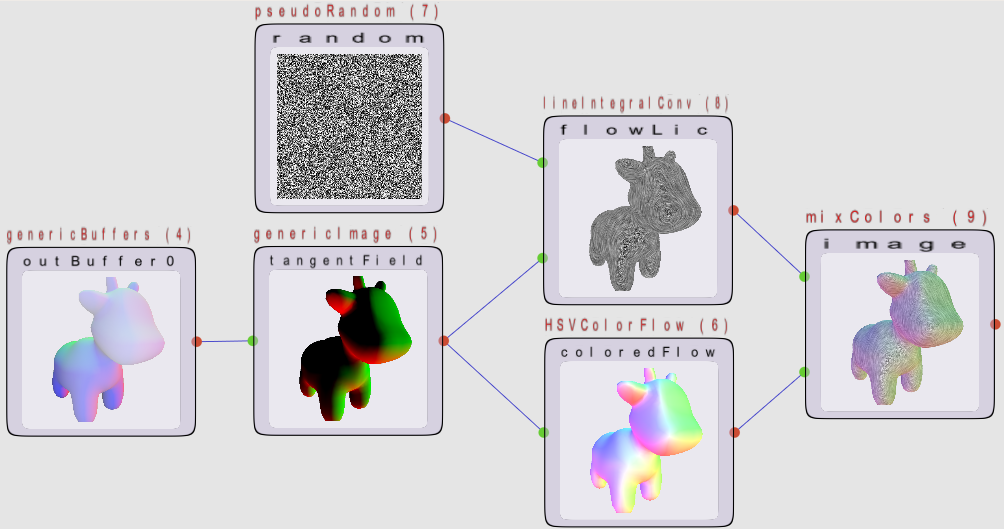
\includegraphics[width=\linewidth]{imgs/pipe-flows.png} 
  \caption{\label{fig:pipe-flow}Flow visualization pipeline example.}
\end{figure}
%
\noindent This pipeline (Fig~\ref{fig:pipe-flow}) illustrates the use of the
``lineIntegralConv'' and the ``HSVColorFlow'' nodes (based in generic
image nodes) to visualize a flow field. In this example, the flow is
obtained by computing the gradient flow of the surface. The line
integral convolution (LIC) blurs a texture (the noise in that case) in
the direction of the flow. This process is commonly used to visualize
flow field. The HSV color node has the same goal, but the input flow
direction is visualized with different hues and magnitude is related
to the color value. The last node on the right combines the flow to
obtain an original visualization.  The pipeline contains a second
example where an image is abstracted by applying a LIC, based on its
gradient flow.

\newpage
\addsubsection{laplacian-pyramid.gra}
\noindent The laplacian example (Fig.~\ref{fig:pipe-pyr}) shows how to use the
gaussian and laplacian pyramid nodes to decompose and modify the
frequency components of an image before rebuilding it. These pyramids
are all based on the ``genericPyramid'' node. In this example, small
scale details are enhanced before reconstructing the image. The last
node shows the resulting enhanced image by selecting the finest scale
of the pyramid (in a generic image node).

%
\begin{figure}[h!]
  \centering 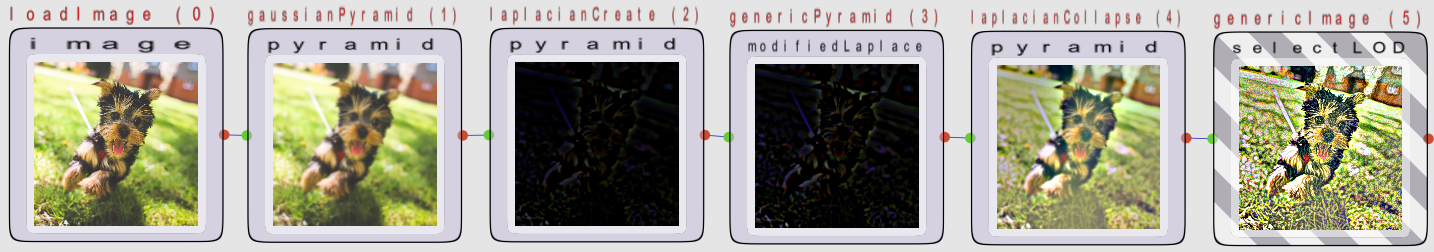
\includegraphics[width=\linewidth]{imgs/pipe-pyr.png} 
  \caption{\label{fig:pipe-pyr}Laplacian pyramid pipeline example.}
\end{figure}
%
\newpage

\addsubsection{global-values.gra}
%
\begin{figure}[htb]
  \centering 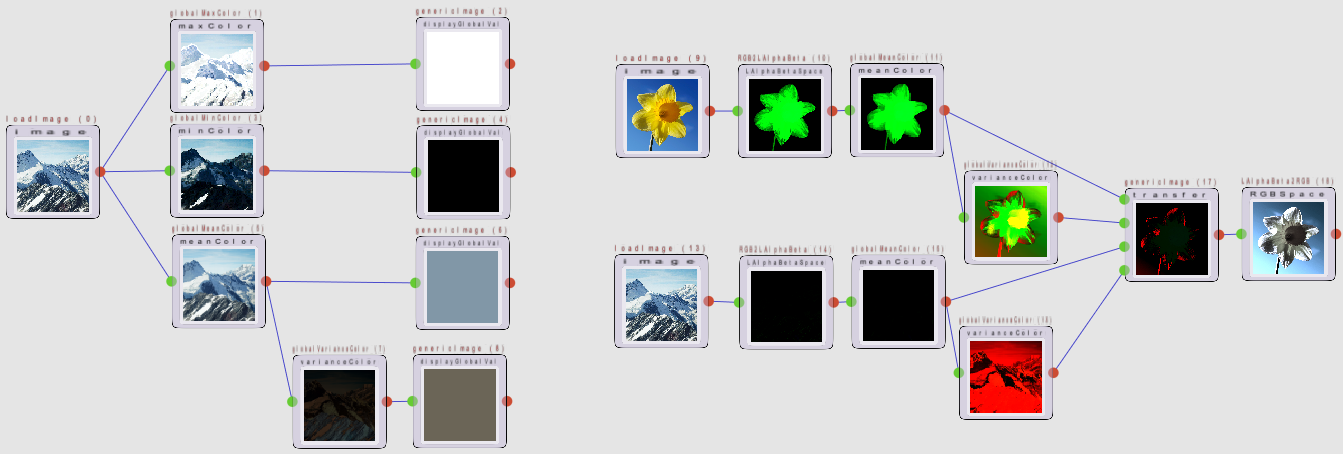
\includegraphics[width=\linewidth]{imgs/pipe-global.png} 
  \caption{\label{fig:pipe-global}Global values pipeline example.}
\end{figure}
%
\noindent The pipeline shown in Fig.~\ref{fig:pipe-global} also makes use of
pyramid nodes to compute global values on images such as the
minimum/maximum/mean/variance colors. This is shown on the left, where
generic images nodes are used to access the last levels of the
pyramids and visualize the corresponding colors. On the right side,
the mean and standard deviations are used to reshape the histogram of
a source image based on a target one (a simple example-based color
transfer function).

\addsubsection{histograms.gra}
%
\begin{figure}[htb]
  \centering 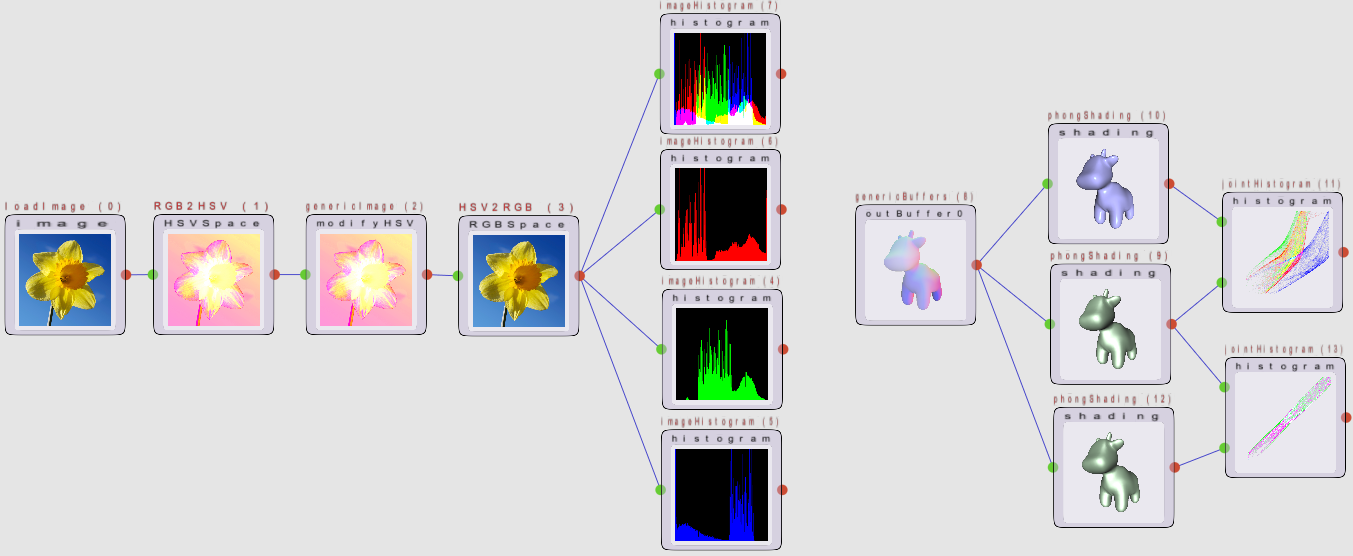
\includegraphics[width=\linewidth]{imgs/pipe-hist.png} 
  \caption{\label{fig:pipe-hist}Histograms pipeline example.}
\end{figure}
%
\noindent Histograms (Fig.~\ref{fig:pipe-hist}) are based on generic splat
nodes. The left side of the figure shows the original node as well as
some variations that select only one particular channel to
display. The geometry shader was slightly modified for this
purpose. Histograms are obtained in real-time. Try to play with the
parameters of the ``modifyHSV'' node to visualize their effects. On
the right side, a joint histogram is used to visualize the
correlations between 2 rendered images.


\addsubsection{poisson-diffusion.gra}
%
\begin{figure}[htb]
  \centering 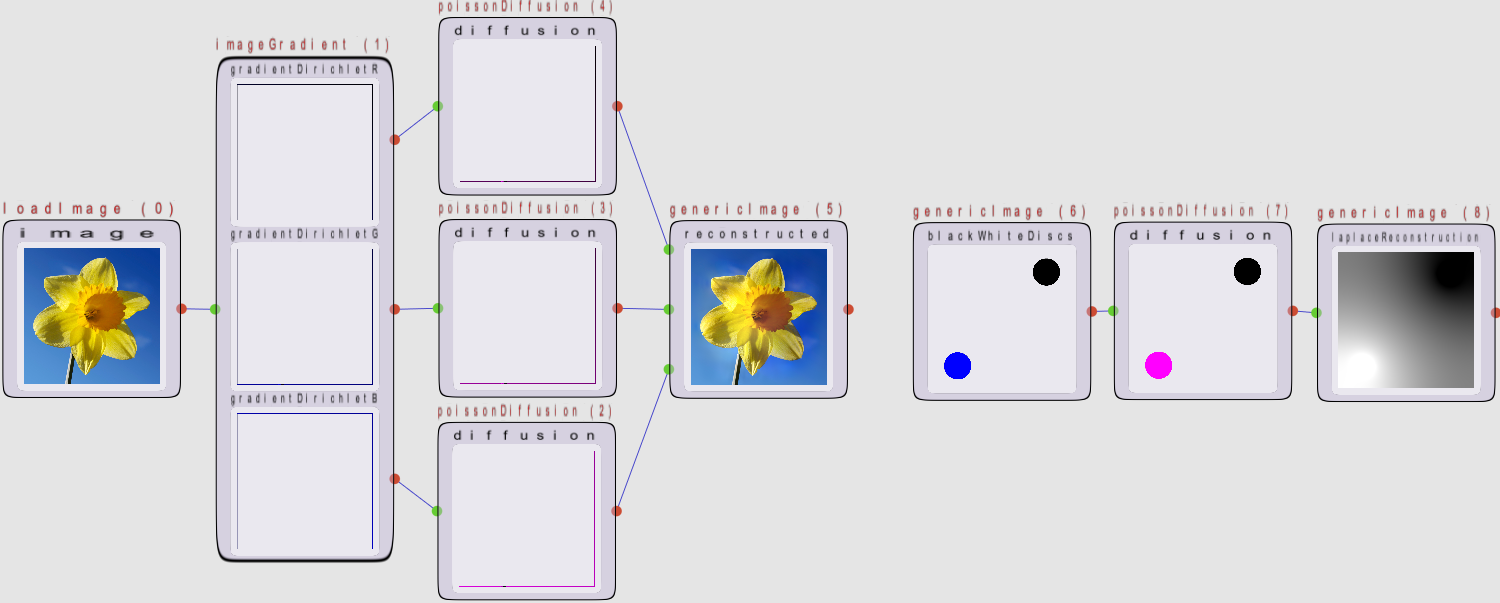
\includegraphics[width=\linewidth]{imgs/pipe-poisson.png} 
  \caption{\label{fig:pipe-poisson}Diffusion pipeline example.}
\end{figure}
%
\noindent The pipeline shown in Fig.~\ref{fig:pipe-poisson} illustrates the use
of the poisson diffusion node to reconstruct an image from its
gradients. On the left, 3 diffusions are computed (one for each
channel) to compute the image. The ``gradientDirichlet node'' is based
on a generic image node and computes the image gradient for each
channel, as well as some Dirichlet constraints on the borders (to
avoid offset differences in the result). The second example on the
right shows how to use the poisson node to compute a laplacian
diffusion. In that case, the gradient is set to 0 everywhere. Only
Dirichlet constraints are placed inside the 2 black/white discs. The
node then diffuses the data by minimizing the gradient. The positions
of the discs can be controlled in real-time in the viewer: click on the
blackWhiteDiscs image, press ``space'' and modify the position of the discs
with the mouse.

\addsubsection{renderings.gra}
%
\begin{figure}[htb]
  \centering 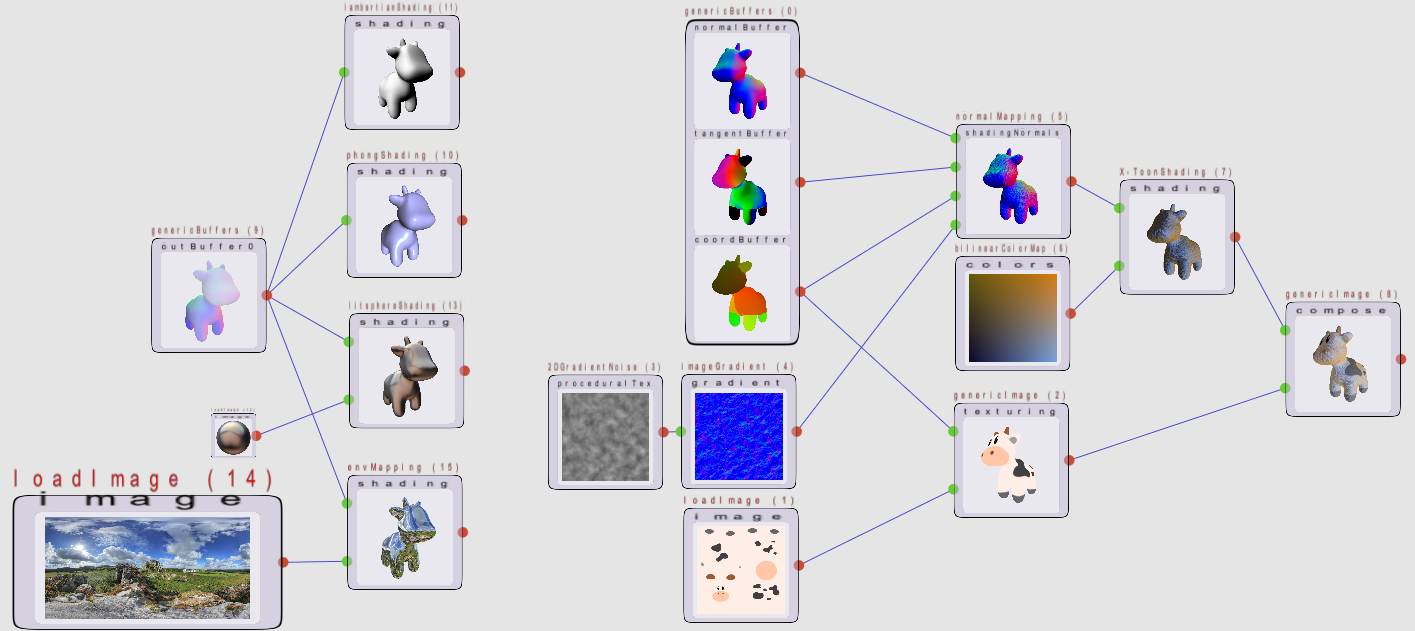
\includegraphics[width=\linewidth]{imgs/pipe-rend.png} 
  \caption{\label{fig:pipe-rend}Renderings pipeline example.}
\end{figure}
%
The rendering pipeline (Fig.~\ref{fig:pipe-rend}) shows the available
shading nodes on the left. They can all be controlled via the mouse
(for moving the light direction) or via some parameters inside the
interface. The right example starts from a generic buffer node for
loading the cow model, and uses the texture coordinates as well as the
tangents in order to perturb normal at the surface (normal-mapping
technique). The model texture is also loaded and combined with a
simple shading to obtain the final result on the right. Parameters for
the normal perturbation, shading colors and textures might be modified
inside the corresponding node interfaces.

\newpage
\addsubsection{displacement-mapping.gra}
%
\begin{figure}[htb]
  \centering 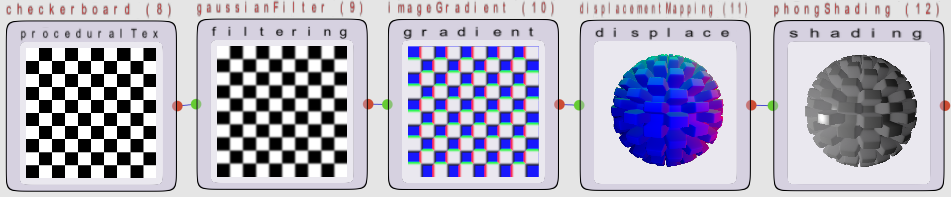
\includegraphics[width=\linewidth]{imgs/pipe-displace.png} 
  \caption{\label{fig:pipe-displace}Displacement mapping pipeline example.}
\end{figure}
%
The displacement mapping technique (Fig.~\ref{fig:pipe-displace})
displaces mesh vertices based on an input height map. Here,
the input texture also contains the associated normals, based on
the gradient of a blurred checkerboard texture. The displacement is
applied on a sphere. The ``disp'' parameter inside the interface of
the displacement node controls how the sphere is deformed. ``T''
controls how the sphere should be tesselated (how many triangles
needed) via the tesselation shader to displace all the details.


\addsubsection{animate.gra}
%%
%\begin{figure}[tbh]
%  \centering 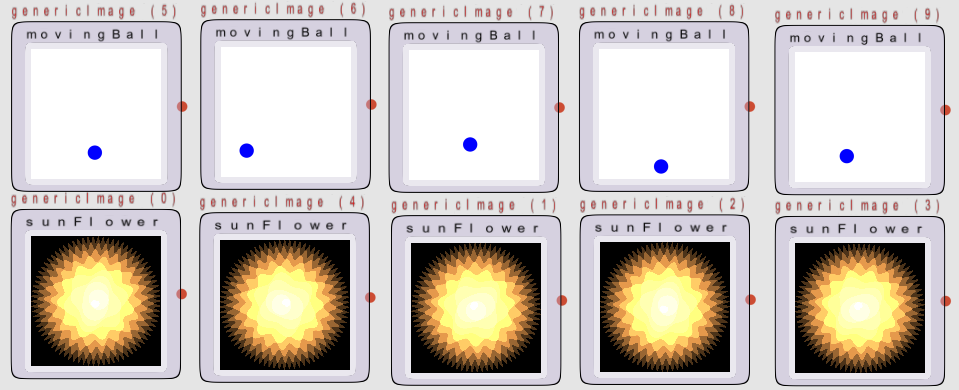
\includegraphics[width=\linewidth]{imgs/pipe-anim.png} 
%  \caption{\label{fig:pipe-anim}The animation pipeline example.}
%\end{figure}
%%
The animation example illustrates basic animation behaviors. 
You will have to open the pipeline to follow the remainder of this section. 
The five nodes on the top row show a disc passing through 4 control points, using five different interpolation types: linear, step, shepard, spline and hermite. 
The second row of nodes shows a rotated sunFlower illustrating the effect of the curve behavior on a small
number of control points: no behavior (all linear), constant, repeat, mirrored repeat and offseted repeat. 
Press the ``p'' key to start the animation and see the effects (press
``shift+p'' to stop it). To check and modify the curves, click on the
editing button of the parameter inside the interface of the node.


\addsubsection{fourier-transform.gra}

\begin{figure}[tbh]
 \centering 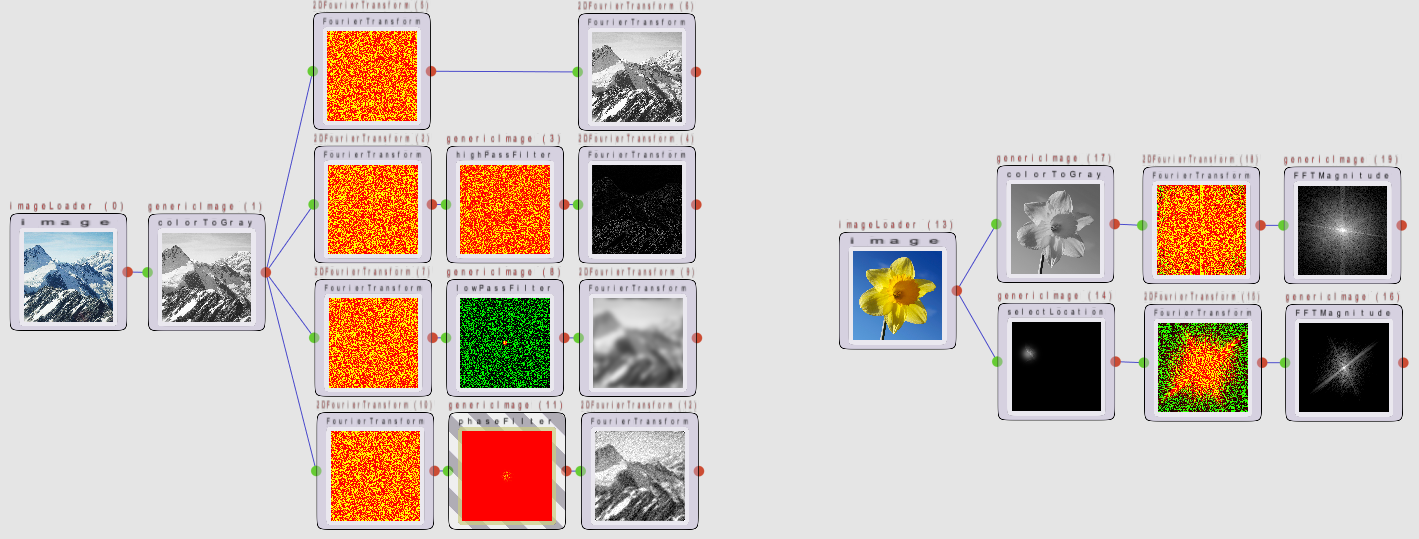
\includegraphics[width=\linewidth]{imgs/pipe-fourier.png} 
 \caption{\label{fig:pipe-fourier}The Fourier pipeline example.}
\end{figure}

The Fourier transform example (Fig.~\ref{fig:pipe-fourier}) shows how
to use the node to manipulate the frequency content in images. On the
left, forward and backward Fourier transforms are successively
applied. From top to bottom: the original image is reconstructed; a
highpass filter is applied (using a genericImage node that multiplies
the frequency magnitude with a user-defined gaussian function); a
low-pass filter is applied (on the magnitude - same approach); a
low-pass filter is applied (on the phase - same approach). On the
right, the magnitude is rescaled using a generic node to visualize the
spectrum. (top) the full spectrum is visualized; (bottom) the user can
interact with the select node (click + space on the node and interact
in the viewer) to visualize the spectrum of a part of the image only.



%% \small{
%% \bibliographystyle{alpha}
%% \bibliography{guide}
%% }
\end{document}

